\documentclass[tikz,border=6pt]{standalone}
\usepackage{xcolor}
\usetikzlibrary{arrows.meta,decorations.pathmorphing,calc,positioning,fit,backgrounds,shapes.geometric}
\definecolor{red}{HTML}{A50F2D}\definecolor{ink}{HTML}{141414}\definecolor{gry}{HTML}{5F5F5F}\definecolor{lgry}{HTML}{E6E6E6}
\definecolor{blu}{HTML}{2B6CB0}\definecolor{teal}{HTML}{1B9E8F}\definecolor{org}{HTML}{E8702A}\definecolor{grn}{HTML}{2E9E5B}\definecolor{mag}{HTML}{D81B60}\definecolor{pur}{HTML}{5B2C83}
\tikzset{fibre/.style={ink,line width=1.6pt,line cap=round},
 sis1/.style={org,line width=1.8pt,line cap=round},sis2/.style={blu,line width=1.8pt,line cap=round},
 lab/.style={font=\sffamily\small,text=ink},lbl/.style={font=\sffamily\footnotesize,text=gry,align=center},ttl/.style={font=\sffamily\bfseries\small,text=ink},
 ctcf/.style={-{Triangle[length=5pt,width=6pt]},pur,line width=2.4pt},
 cohesin/.style={grn,line width=1.6pt}}

% ---- shared drawing macros: a DNA duplex is a dark tube with a light core
\newcommand{\dx}[2][ink]{\draw[line width=3.6pt,#1,line cap=round] #2; \draw[line width=1.3pt,white,line cap=round] #2;}
% omega-shaped loop: base at (x,y), radius r
\newcommand{\omegapath}[3]{(#1-0.35,#2) .. controls (#1-0.35,#2+0.45) and (#1-#3,#2+0.35) .. (#1-#3,#2+#3+0.45) arc[start angle=180,end angle=0,radius=#3] .. controls (#1+#3,#2+0.35) and (#1+0.35,#2+0.45) .. (#1+0.35,#2)}
% replication eye: origin at (x,y), half width w, half height h
\newcommand{\eyetop}[4]{(#1-#3,#2) .. controls (#1-#3*0.5,#2+#4*1.33) and (#1+#3*0.5,#2+#4*1.33) .. (#1+#3,#2)}
\newcommand{\eyebot}[4]{(#1-#3,#2) .. controls (#1-#3*0.5,#2-#4*1.33) and (#1+#3*0.5,#2-#4*1.33) .. (#1+#3,#2)}
\newcommand{\eye}[4]{\dx[org]{\eyetop{#1}{#2}{#3}{#4}}\dx[blu]{\eyebot{#1}{#2}{#3}{#4}}\fill[teal] (#1-#3,#2) circle (3.2pt) (#1+#3,#2) circle (3.2pt);}
% cohesin ring that ENCIRCLES DNA: back half drawn before the DNA, front half after it
% flat ring around a pair of stems (loop base): x, y, half width
\newcommand{\rg}[1]{\draw[line width=3.4pt,grn!80!black,line cap=round] #1; \draw[line width=1.3pt,grn!25!white,line cap=round] #1;}
\newcommand{\ringbb}[3]{\rg{(#1-#3,#2) arc[start angle=180,end angle=0,x radius=#3,y radius=0.2]}}
\newcommand{\ringbf}[3]{\rg{(#1-#3,#2) arc[start angle=180,end angle=360,x radius=#3,y radius=0.2]}}
% tall ring around horizontal fibre(s): x, y centre, half height
\newcommand{\ringvb}[3]{\rg{(#1,#2+#3) arc[start angle=90,end angle=270,x radius=0.17,y radius=#3]}}
\newcommand{\ringvf}[3]{\rg{(#1,#2-#3) arc[start angle=-90,end angle=90,x radius=0.17,y radius=#3]}}
% omega loop with base half width w
\newcommand{\omegaw}[4]{(#1-#4,#2) .. controls (#1-#4,#2+0.45) and (#1-#3,#2+0.35) .. (#1-#3,#2+#3+0.45) arc[start angle=180,end angle=0,radius=#3] .. controls (#1+#3,#2+0.35) and (#1+#4,#2+0.45) .. (#1+#4,#2)}
\newcommand{\gseg}[3]{\dx[gry]{(#2,#1) -- (#3,#1)}}

\begin{document}
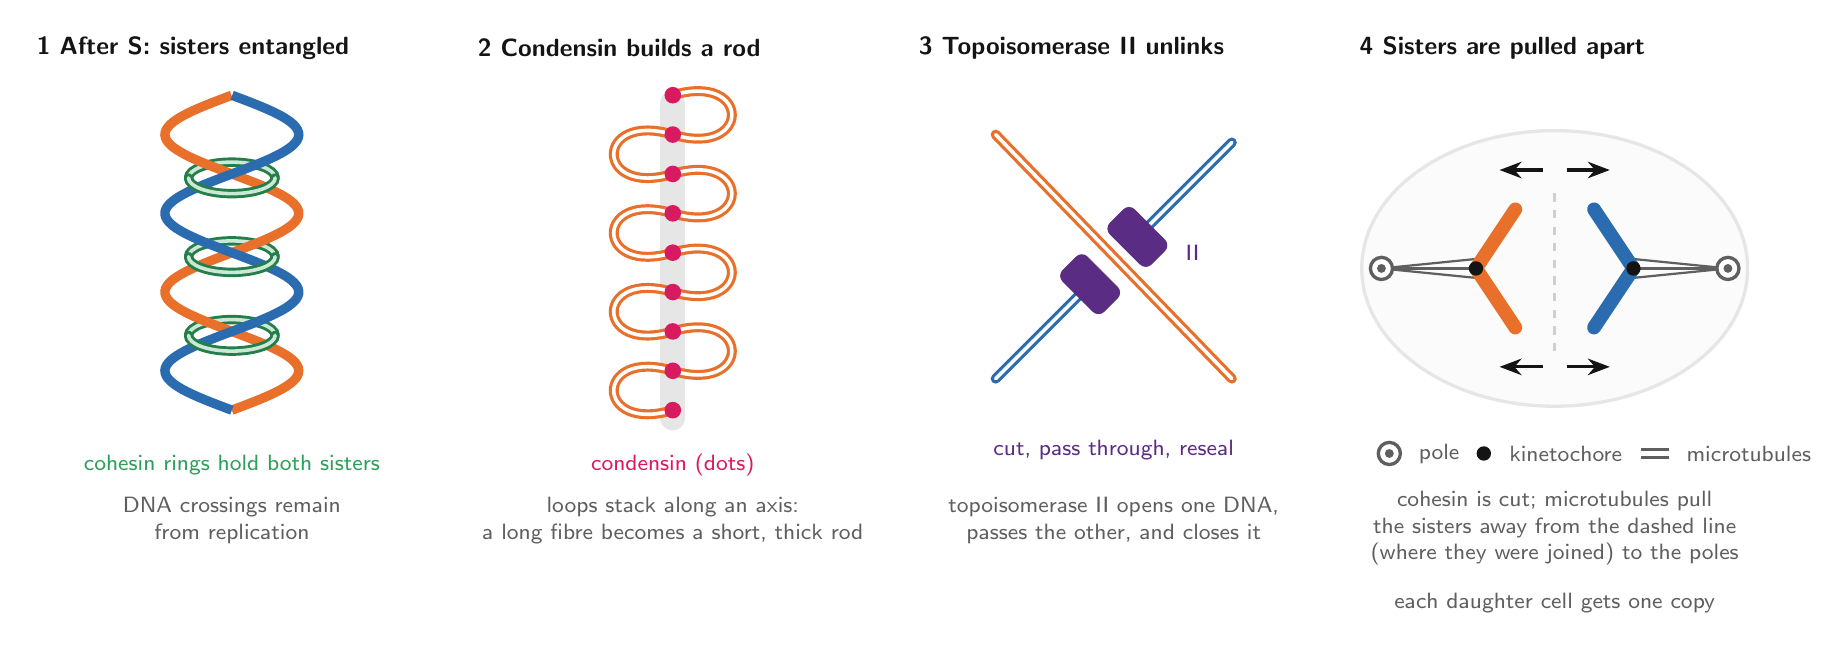
\begin{tikzpicture}[font=\sffamily\small,>=Stealth]
\foreach \x/\t in {0/{1  After S: sisters entangled},5.6/{2  Condensin builds a rod},11.2/{3  Topoisomerase II unlinks},16.8/{4  Sisters are pulled apart}}{\node[ttl,anchor=west] at (\x,4.6) {\t};}
% 1 : two duplexes twisted around each other, cohesin rings
\begin{scope}[xshift=1.4cm]
 \foreach \y in {1,2,3}{\ringbb{1.2}{\y-0.05}{0.55}}
 \draw[org,line width=3.4pt,domain=0:4,samples=120,smooth,variable=\y] plot ({0.85*sin(180*\y)+1.2},\y);
 \draw[blu,line width=3.4pt,domain=0:4,samples=120,smooth,variable=\y] plot ({-0.85*sin(180*\y)+1.2},\y);
 \foreach \y in {1,2,3}{\ringbf{1.2}{\y-0.05}{0.55}}
 \node[lbl,grn] at (1.2,-0.7) {cohesin rings hold both sisters};
 \node[lbl] at (1.2,-1.4) {DNA crossings remain\\ from replication};
\end{scope}
% 2 : central axis with condensin-made loops on both sides
\begin{scope}[xshift=8.2cm]
 \draw[line width=9pt,lgry,line cap=round] (0,-0.1) -- (0,3.9);
 % one continuous fibre: loops alternate left and right, stacked along the axis
 \dx[org]{(0,0) \foreach \y/\s in {0/-1,0.5/1,1.0/-1,1.5/1,2.0/-1,2.5/1,3.0/-1,3.5/1}{.. controls (\s*1.0,\y-0.3) and (\s*1.0,\y+0.8) .. (0,\y+0.5)}}
 \foreach \y in {0,0.5,1.0,1.5,2.0,2.5,3.0,3.5,4.0}{\fill[mag] (0,\y) circle (3pt);}
 \node[lbl,mag] at (0,-0.7) {condensin (dots)};
 \node[lbl] at (0,-1.4) {loops stack along an axis:\\ a long fibre becomes a short, thick rod};
\end{scope}
% 3 : topoisomerase II passes one duplex through a cut in the other
\begin{scope}[xshift=12.3cm]
 \dx[blu]{(0,0.4) -- (1.2,1.6)} \dx[blu]{(1.8,2.2) -- (3.0,3.4)}
 \foreach \p in {(1.2,1.6),(1.8,2.2)}{\node[fill=pur,rounded corners=3pt,rotate=45,minimum width=0.45cm,minimum height=0.75cm] at \p {};}
 \dx[org]{(0,3.5) -- (3.0,0.4)}
 \node[lbl,pur] at (2.5,2.0) {II};
 \node[lbl,pur] at (1.5,-0.5) {cut, pass through, reseal};
 \node[lbl] at (1.5,-1.4) {topoisomerase II opens one DNA,\\ passes the other, and closes it};
\end{scope}
% 4 : anaphase: cohesin cut, each sister is pulled to its own pole
\begin{scope}[xshift=17.65cm]
 \draw[lgry,line width=1.2pt,fill=lgry!15] (1.75,1.8) ellipse (2.45 and 1.75);
 % spindle poles, microtubules (fan from pole to kinetochore), kinetochores
 \foreach \p/\k/\d in {-0.45/0.75/1,3.95/2.75/-1}{
   \foreach \a in {-0.12,0,0.12}{\draw[gry,line width=0.8pt] (\p,1.8) -- (\k,1.8+\a);}
   \draw[gry,line width=1.2pt,fill=white] (\p,1.8) circle (4pt); \fill[gry] (\p,1.8) circle (1.6pt);}
 % sister chromatids: V shapes, centromere (kinetochore) towards the pole
 \draw[org,line width=5pt,line cap=round,line join=round] (1.25,2.55) -- (0.75,1.8) -- (1.25,1.05);
 \draw[blu,line width=5pt,line cap=round,line join=round] (2.25,2.55) -- (2.75,1.8) -- (2.25,1.05);
 \fill[ink] (0.75,1.8) circle (2.6pt) (2.75,1.8) circle (2.6pt);
 % movement: pairs of arrows away from the former metaphase plate (dashed)
 \draw[lgry!90!black,dashed,line width=0.9pt] (1.75,0.75) -- (1.75,2.85);
 \foreach \y in {3.05,0.55}{\draw[->,ink,line width=1.1pt] (1.6,\y) -- (1.05,\y); \draw[->,ink,line width=1.1pt] (1.9,\y) -- (2.45,\y);}
 % legend with the three symbols, evenly spaced
 \draw[gry,line width=1.2pt,fill=white] (-0.35,-0.55) circle (4pt); \fill[gry] (-0.35,-0.55) circle (1.6pt); \node[lbl,anchor=west] at (-0.1,-0.55) {pole};
 \fill[ink] (0.85,-0.55) circle (2.6pt); \node[lbl,anchor=west] at (1.05,-0.55) {kinetochore};
 \draw[gry,line width=0.8pt] (2.85,-0.5) -- (3.2,-0.5) (2.85,-0.6) -- (3.2,-0.6); \node[lbl,anchor=west] at (3.3,-0.55) {microtubules};
 \node[lbl] at (1.75,-1.5) {cohesin is cut; microtubules pull\\ the sisters away from the dashed line\\ (where they were joined) to the poles};
 \node[lbl] at (1.75,-2.45) {each daughter cell gets one copy};
\end{scope}
\end{tikzpicture}
\end{document}
